%
The linear phase is succeeded by a transition phase to the saturated phase.
In this phase, the linear modes become large enough for non-linear effects to affect the dynamics of the system.
We will start this chapter by briefly explain how this interaction brings the system into the saturated steady state.

\section{Transition to saturated turbulence}
Through the non-linear interactions (in particular through the non-linear advective terms) energy from the unstable, growing modes spreads to neighboring modes in the $k$-spectrum.
This can be seen around $t=0.0175\s$ in \cref{fig:fourierUnstable}, where $m_\theta=1$ suddenly shows a growth with a higher growth rate than the rest of the modes.
The transfer of energy can by studied through three-wave coupling under the assumptions that only neighboring modes in the $k$-spectrum interact (the weak turbulence assumption), and that four-wave and higher-wave couplings are negligible.
This has been done in for example \cite{Ritz1989,Knorr1990}.

The cascading of energy through the different modes is what eventually brings the system into a saturated turbulence phase.
In an attempt to describe how this happens, an idealized case of fluid turbulence was considered by Kolmogorov and Oboukhov in their $1941$ theory of turbulence \cite{Kolmogorov1962}.
The main assumptions of the theory is that the energy fed into the system in a narrow range of $k$, and that the dissipation of energy only happens at the smallest scales, which (in the $k$-spectrum) is well separated from the injection of energy.
In other words, there will be a mechanism feeding the turbulence with structures of a certain size.
These structures break up into smaller structures (the energy is cascading to higher $k$), which again break up into smaller structures, all the way until a viscous sink removes the energy from the system.
The famous decay rate $\propto k^{-5/3}$ is then found for the energy through dimensional arguments.

If the system is constrained to two effective dimension, the system can display an inverse cascade of the energy \cite{Kraichan1980}.
This means that energy can be fed into the system at one range, and it will grow until some mechanis removes the energy at a macroscopic scale.
The inverse energy cascade discussed in \cite{Kraichan1980} is a consequence of the fact that the enstrophy (global integrated vorticity) and energy is conserved simultaneously.
The analysis predicts a decay rate $\propto k^{-5/3}$ for the enstrophy, and a decay rate of $\propto k^{-3}$ for the energy.
In the $2$-D turbulence, structures are allowed to merge together and form larger structures as vortex stretching cannot occur in the system \cite{Fjortoft1953}.
The analysis of the cascading property becomes complicated if dissipations are allowed in the system so that the energy and the enstrophy is not conserved.
It becomes even more complicated if the system is allowed to have some dynamics in the third dimension.
In a quasi $2$-D system, there is still is energy cascading towards the smaller structures.
However, if the dynamics for some reason is constrained in one dimension, an inverse cascade of energy can be observed.
For example can the Earth's atmosphere be considered as almost $2$-dimensional as heigth of the atmosphere is small compared to the longitudal and latitudinal dimension, and an inverse cascade of energy is observed in for example \cite{Smith2002}.

The turbulence in a plasma displays a more complex behavior than the turbulence in a neutral fluids due to more degrees of freedom through the electromagnetic forces.
Despite of this, the plasma turbulence shares many of the cascading properties found in neutral fluid turbulence.
Although the decay rates vary, a cascading behavior from an initial range to a dissipative range is found.
In addition, a $2$-D cascading behavior can occur if the plasma is strongly magnetized as this introduces a dimensional anisotropy.
Due to the magnetic field, the perpendicular displacement of fluid parcels is much more restricted than the displacement along the field lines.
The $2$-D turbulence in plasma physics arises naturally from models like the Charney-Hasegawa-Mima model \cite{Boffetta2002} and Hasegawa-Wakatani \cite{Manz2009}, and has also been observed experimentally in linear machines \cite{Tynan2006a}.

The turbulence will reach a steady state once the input of energy through the source is balanced by the dissipation of energy.
On the transition from the quasi-linear phase to the turbulent phase an overshoot in the energy is observed (see \cref{fig:energyTrace008}).
%
\begin{figure}[htb]
    \centering
    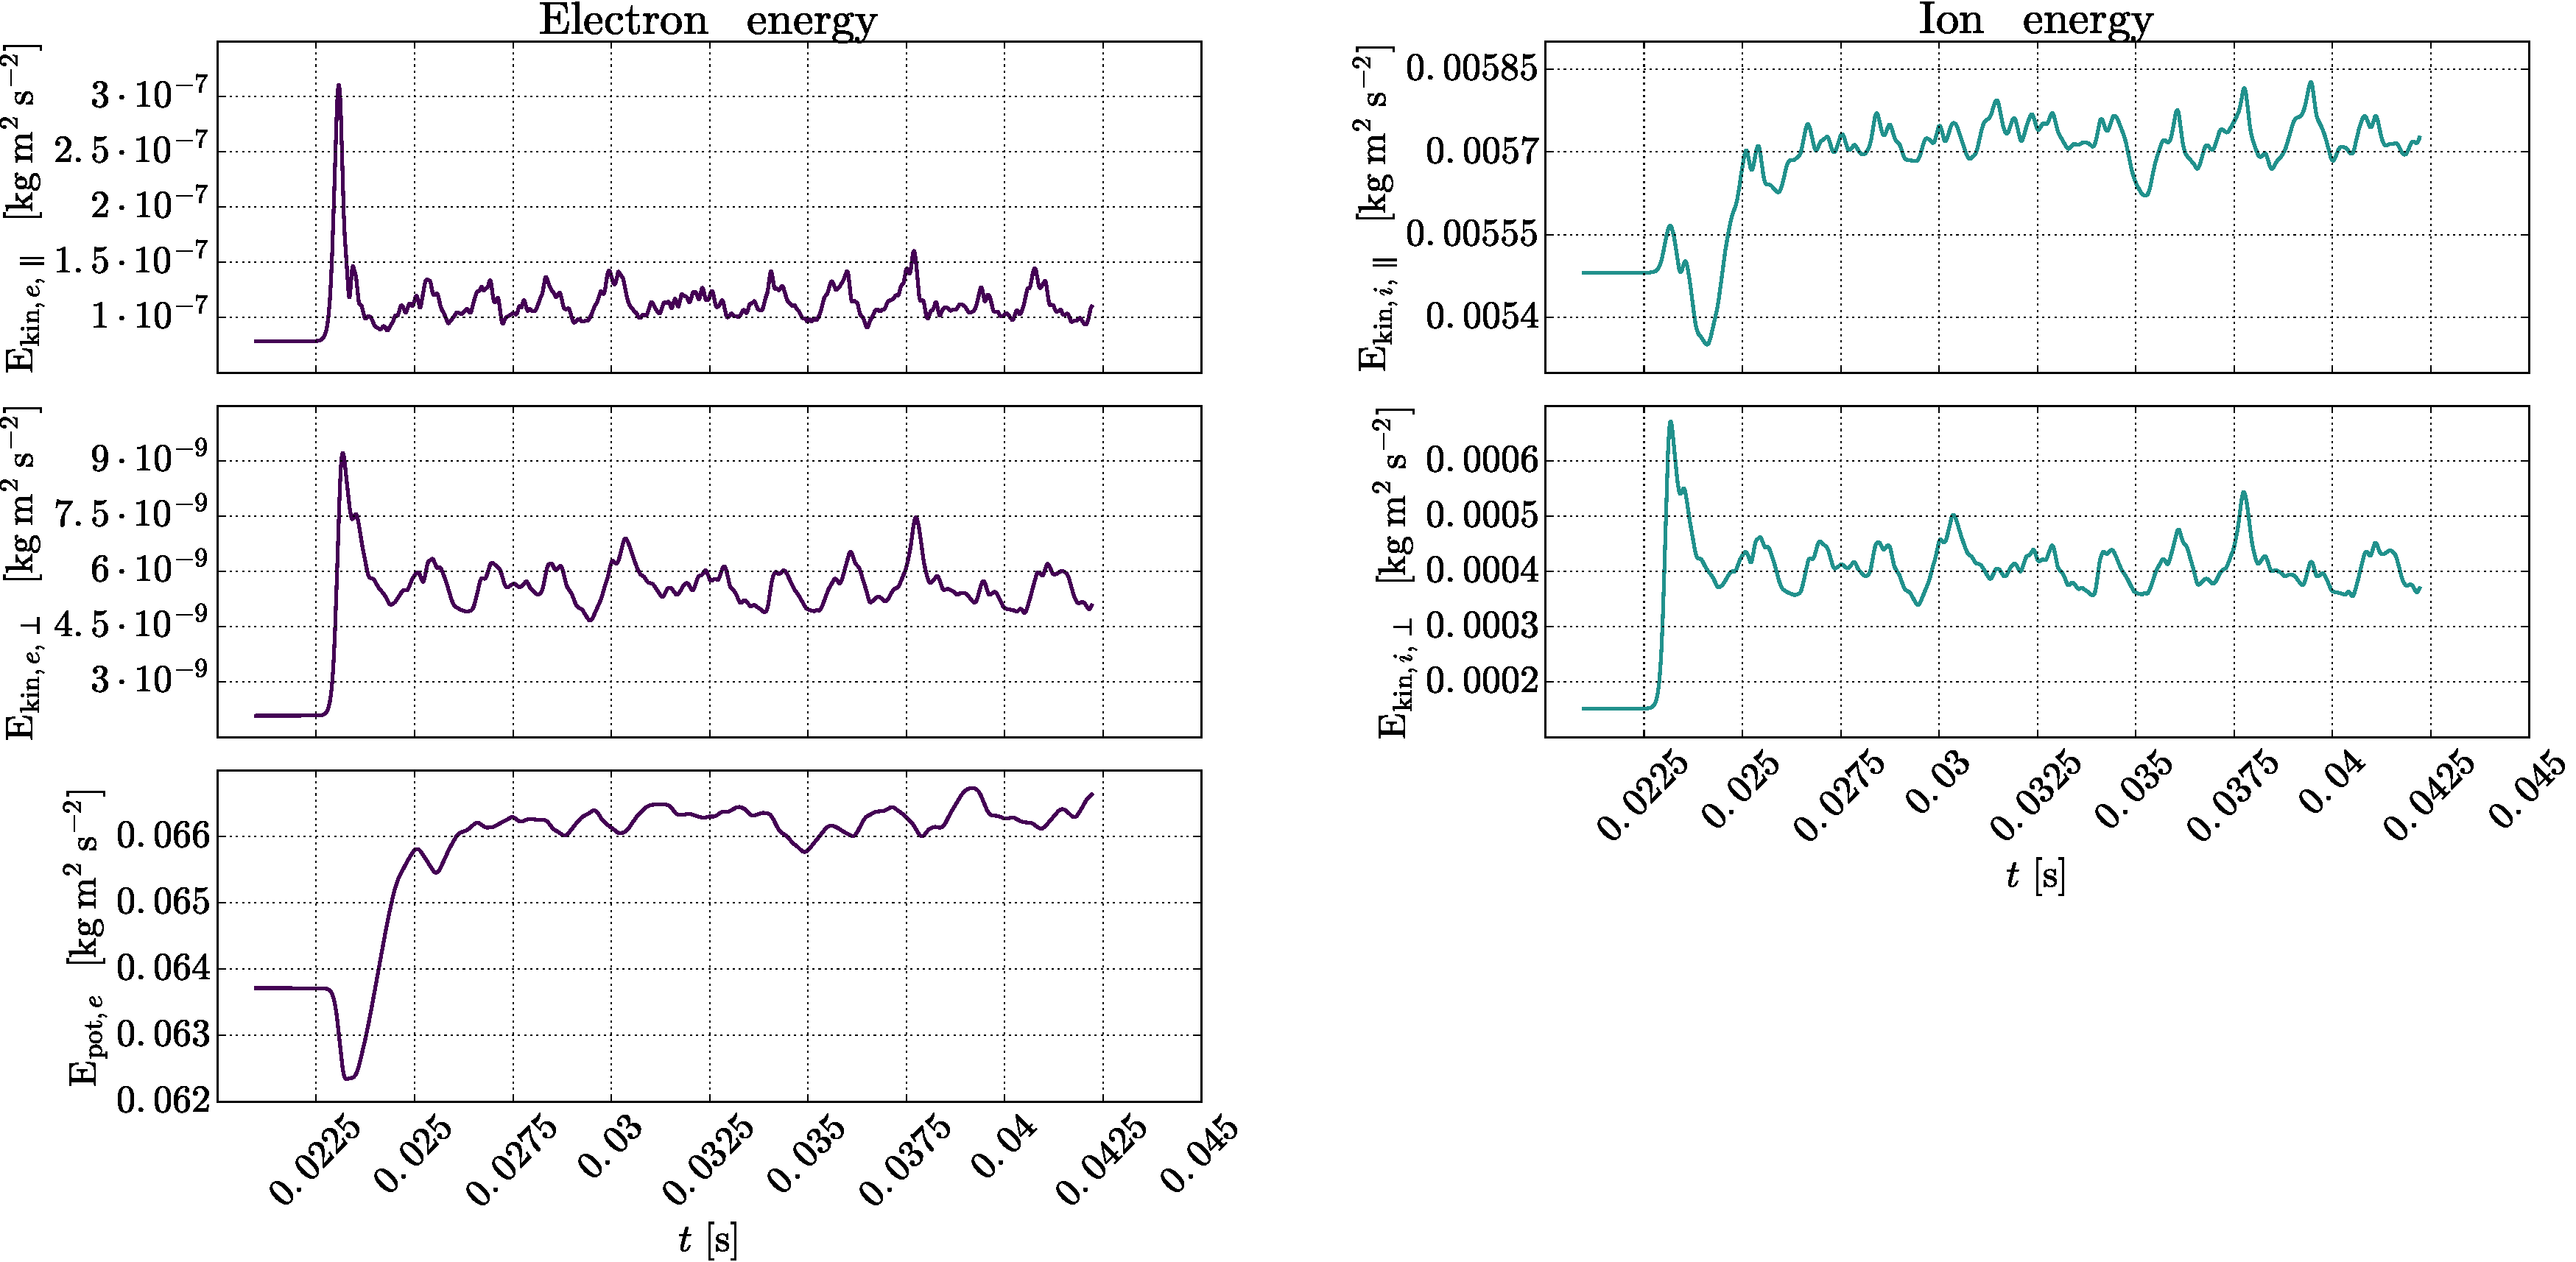
\includegraphics{fig/results/energyTrace/energyTraceB008}
    \caption{Time trace of the energy for $B=0.08\T$.}
    \label{fig:energyTrace008}
\end{figure}
%
As a consequence the eddies evolve at a faster pace at the transition as compared with the saturated turbulent state.
In order to exclude the effects of the transients, we define the start of the saturated turbulence as sometime after the overshoot, around the time where the parallel ion energy is approaching the mean of the rest of the time series.

In the saturated turbulence state, the fluctuations are no longer in an ordered pattern as they were in the linear phase (as shown in \cref{fig:2DFluct}).
%
\begin{figure}[htb]
    \centering
    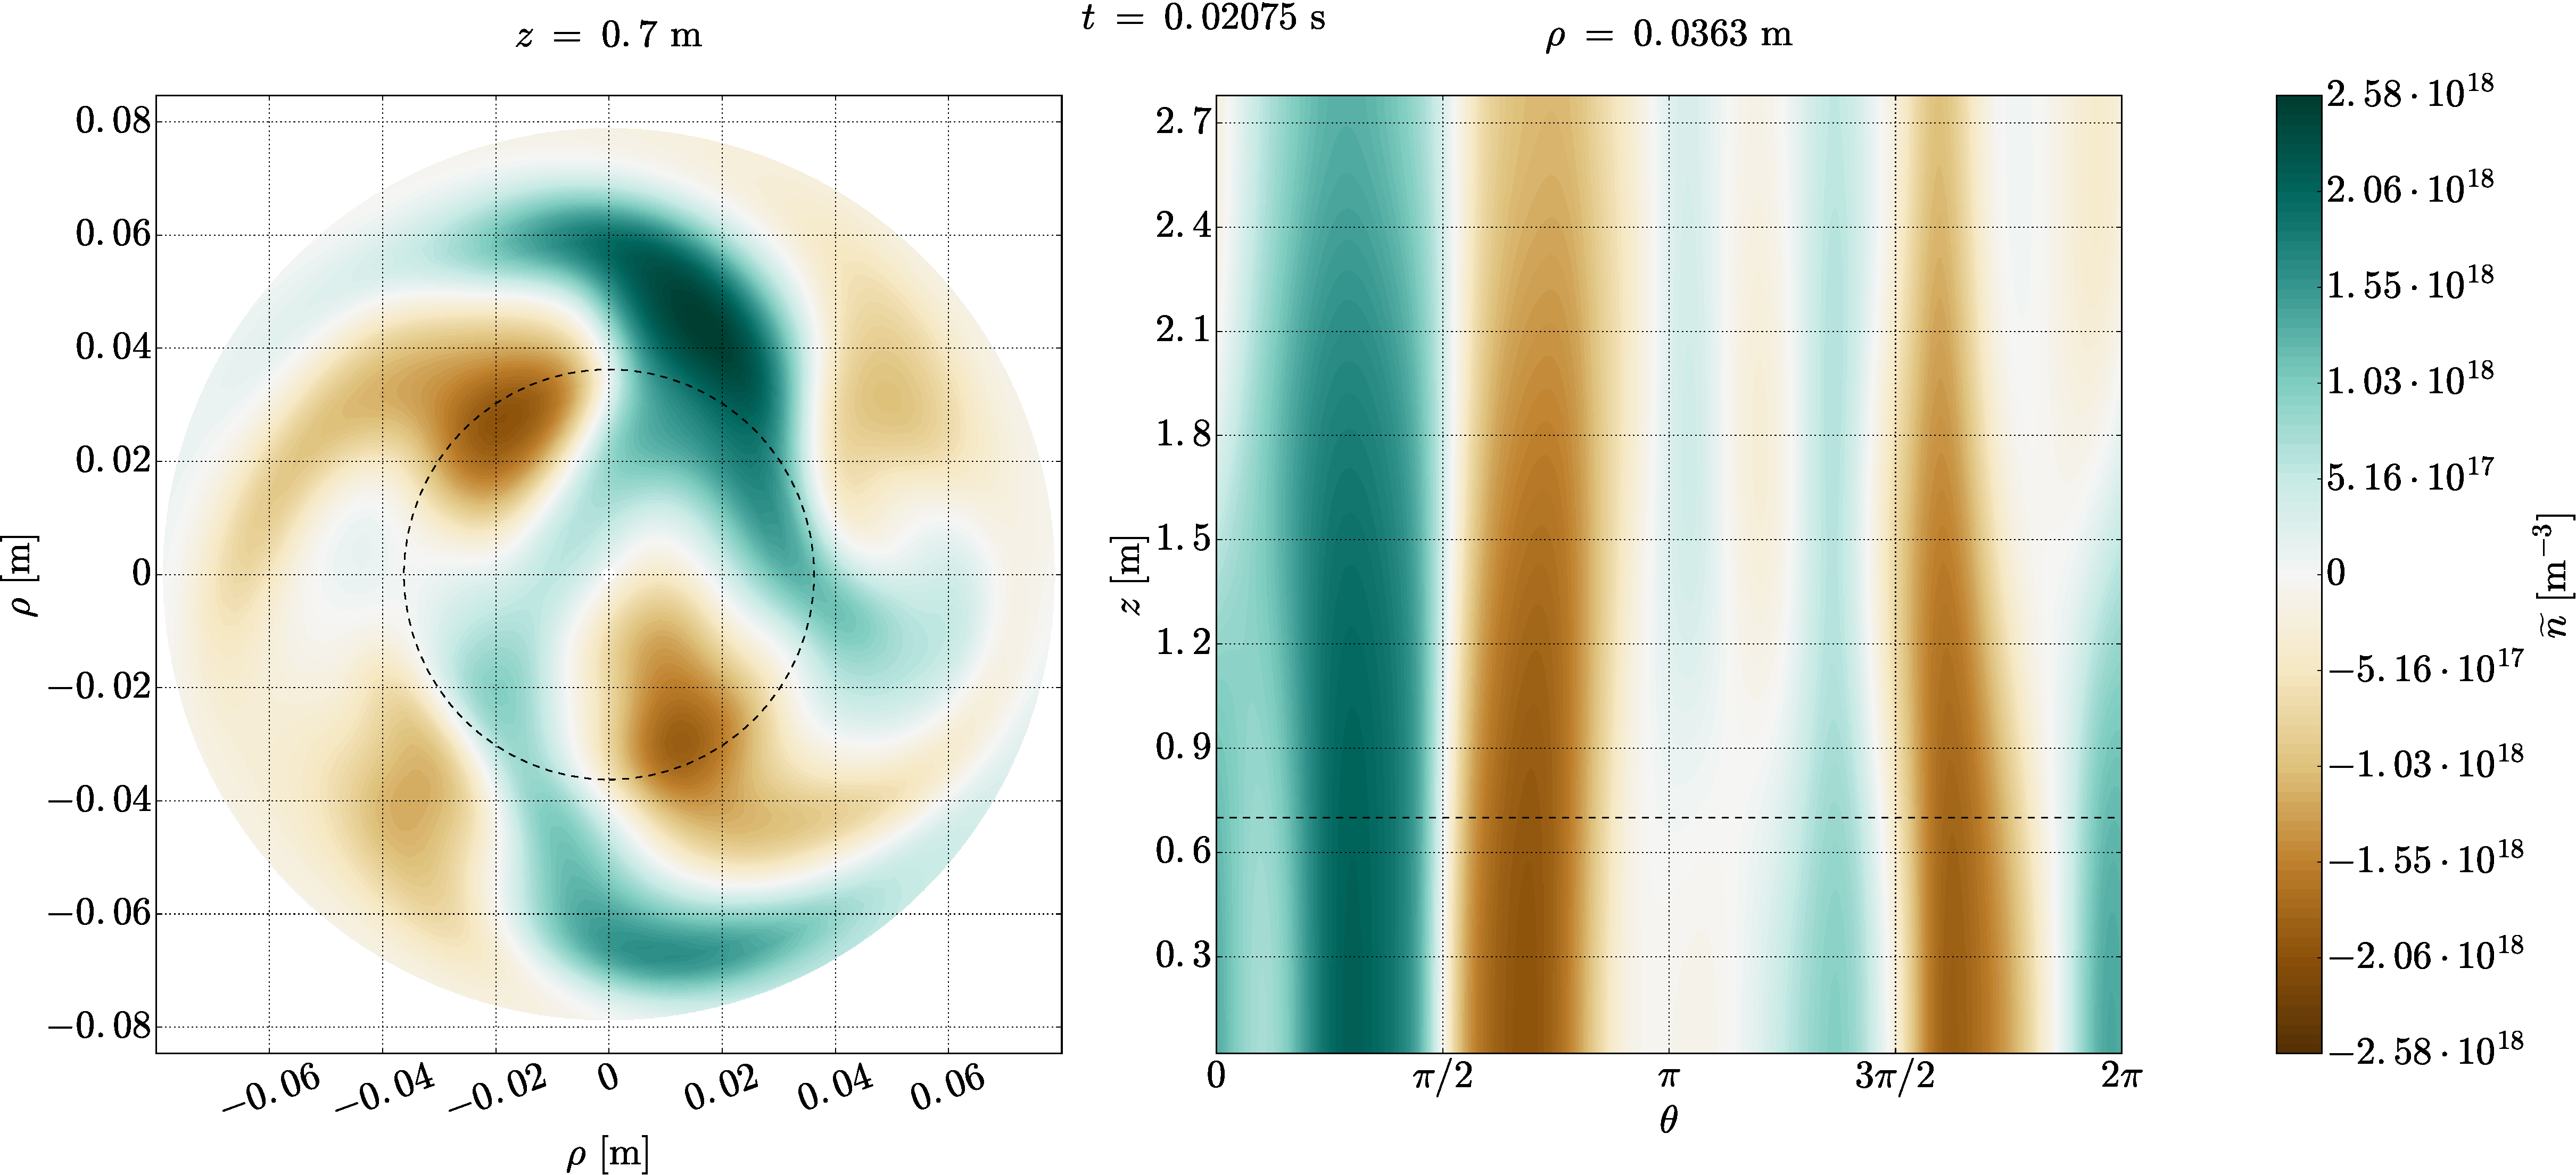
\includegraphics{fig/results/2DTurbulence/fluct}
    \caption{Fluctuations in the turbulent state for $B=0.1\T$.
        The $B$-field points into the paper, and the black dashed lines indicates the slicing of the opposite plot.
    }
    \label{fig:2DFluct}
\end{figure}
%
The fluctuations in this state are big enough to push the bulk part of the plasma off-center as observed in the snap-shots of this state in \cref{fig:turbEv}.

Finally, it is important to note that although there might be one dominating instability which causes the onset to turbulence, the characteristic of the turbulence is more or less independent of the onsetting instability.
In other words, one cannot easily extract the cause of the turbulence by looking at the turbulence alone.
%
{
\clearpage
\thispagestyle{empty}
\begin{figure}[htbp]
    \centering
    \begin{subfigure}[h]{1.00\textwidth}
        \centering
        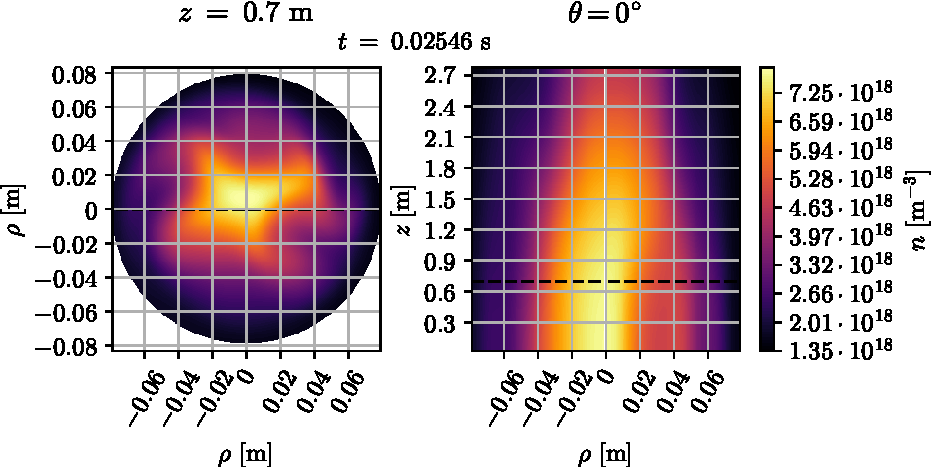
\includegraphics{fig/results/evolution/n-perpPar-2D-0}
    \end{subfigure}%
    \\
    \begin{subfigure}[h]{1.00\textwidth}
        \centering
        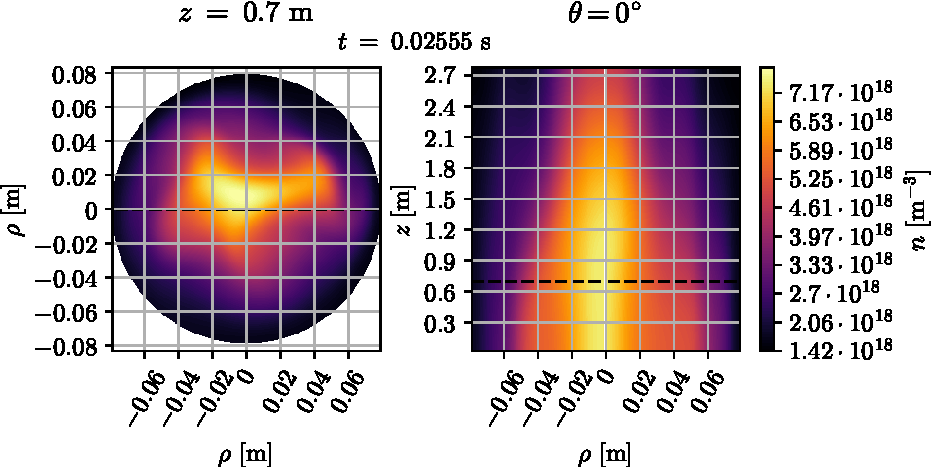
\includegraphics{fig/results/evolution/n-perpPar-2D-1}
    \end{subfigure}
    \\
    \begin{subfigure}[h]{1.00\textwidth}
        \centering
        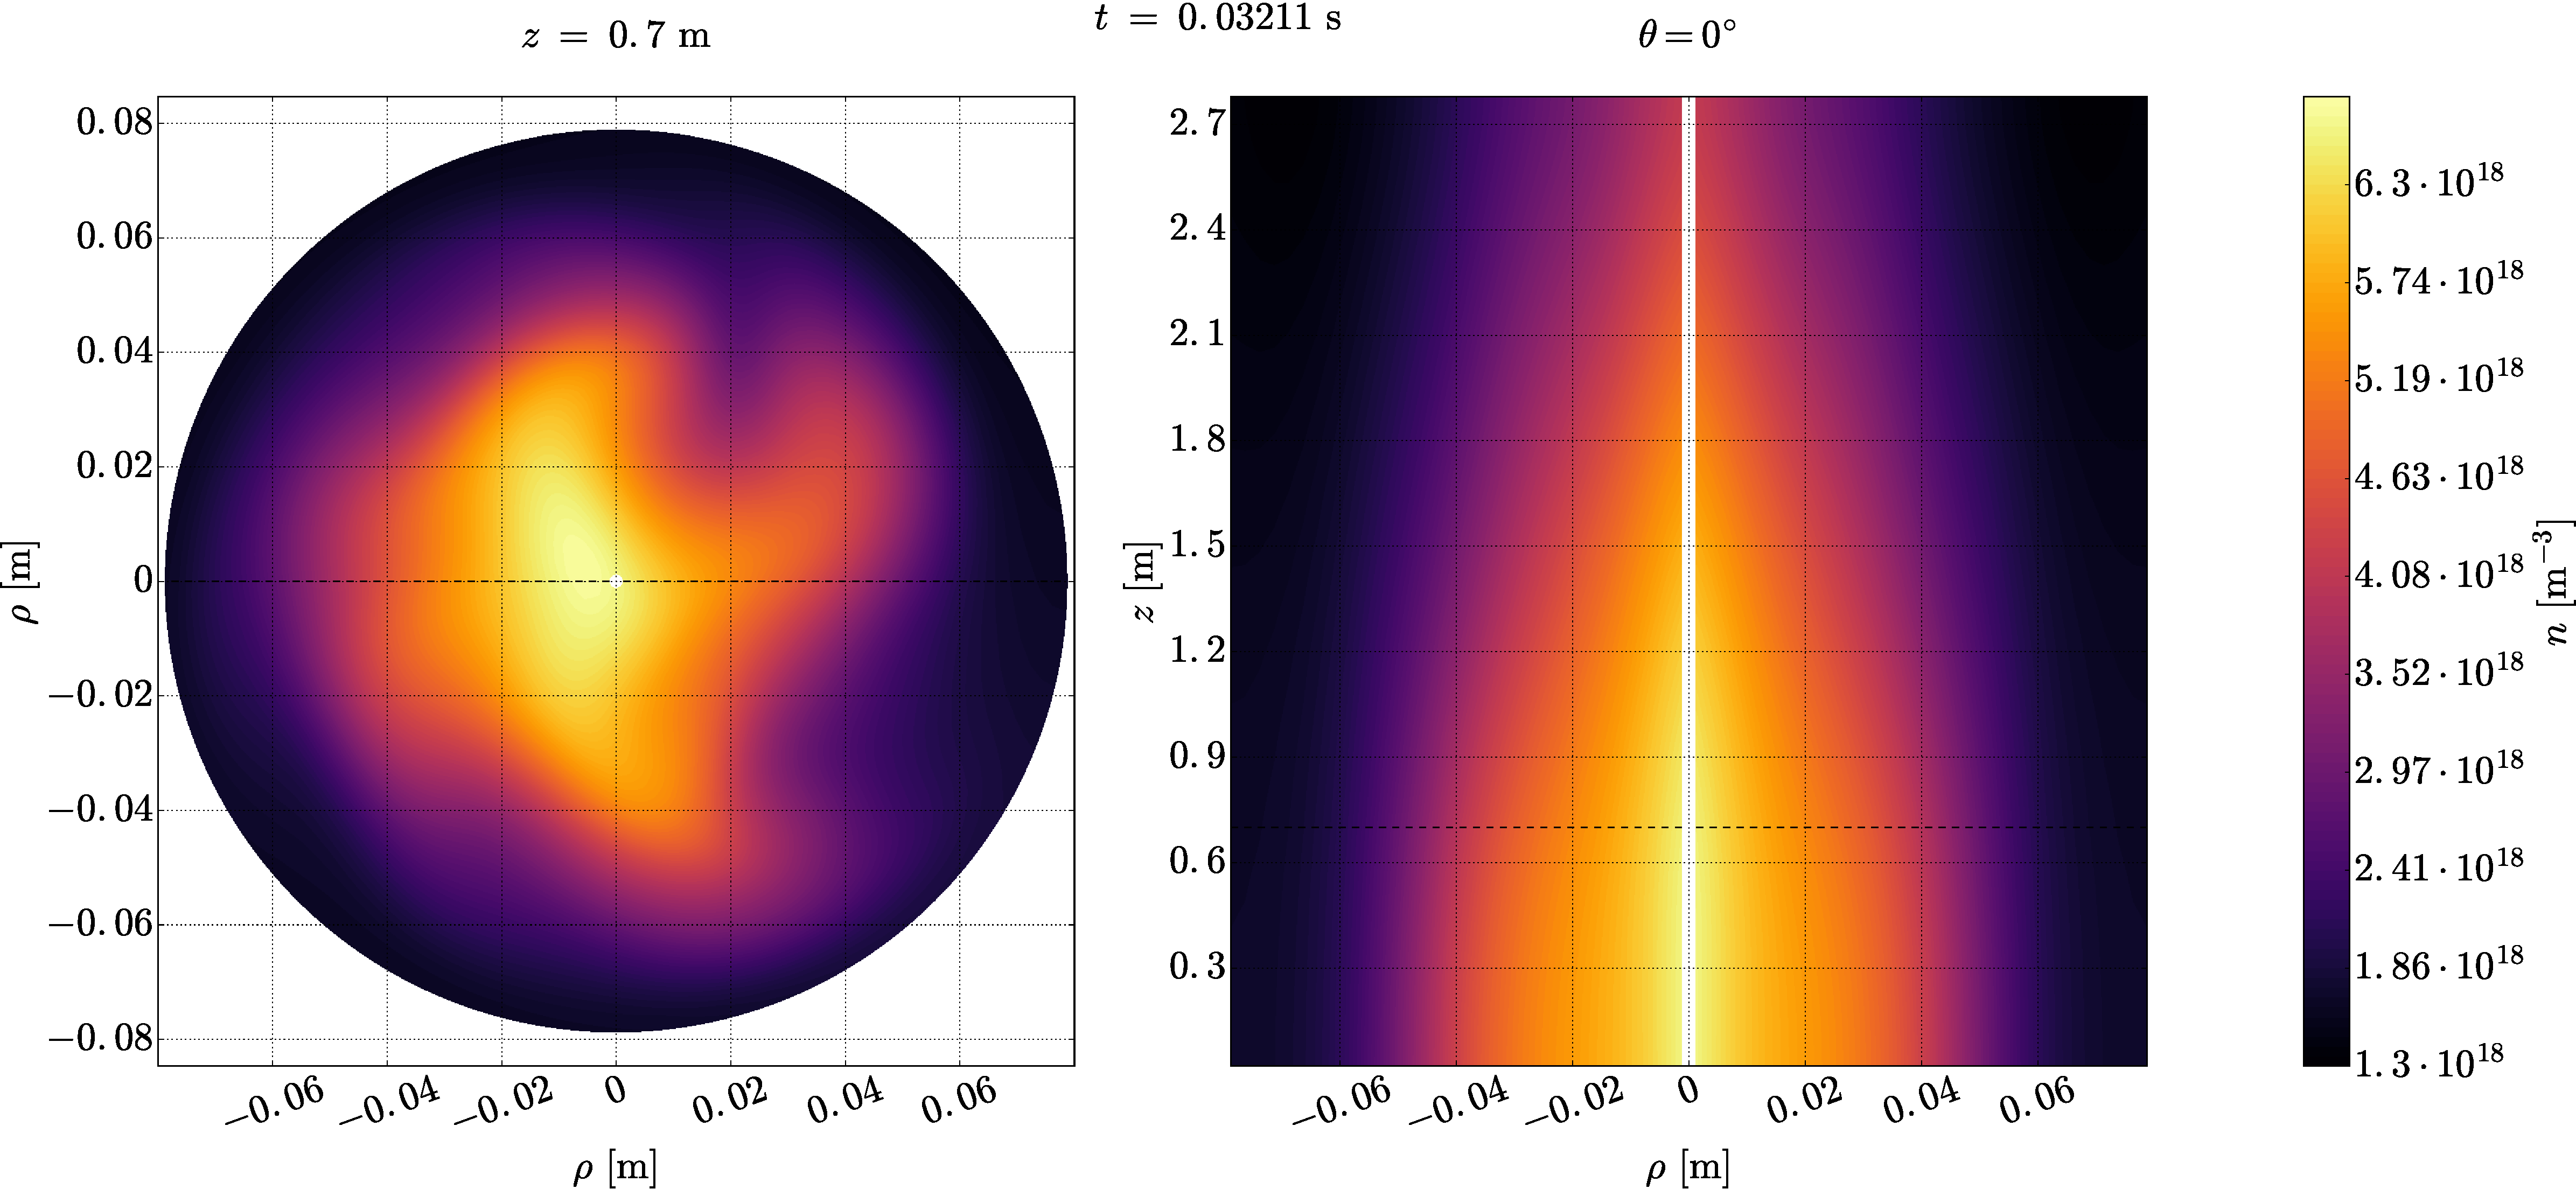
\includegraphics{fig/results/evolution/n-perpPar-2D-2}
    \end{subfigure}
    \caption{Evolution of the plasma in the saturated turbulence phase.
        Here shown for $B=0.1\T$.
        The $B$-field points into the paper, and the black dashed lines indicates the slicing of the opposite plot
    }
    \label{fig:turbEv}
\end{figure}
\clearpage
}
%
